\subsection{Jianhong's summary}
%\subsubsection{Fast AutoAugment}
%
%I tried to reproduce the state-of-the-art result in the paper 'Fast AutoAugment' \cite{lim2019fast}. 
%
%They use the technique of fast auto-augmentation (FAA) to enhance the data in every epoch and get 79.57\% test accuracy with wresnet40x2 for CIFAR-100. Jianqing reproduced the result with 70.63\% test accuracy. Then based on these saved model, I tried to add the the fast auto-augmentation to the test set and evaludate the corresponding test accuracy. For comparison, I also tried to add the very basic augmentation (RandomCrop and RandomHorizontalFlip) to the test set, which is originally used in the training set but not on the test set, for comparison. 
%
%I tested on four models for various augmentation techniques. The results are in the following tables.
%\begin{enumerate}
%\item The best model the paper saved by training with FAA, top1 test=79.57\%
%\item The best model Jianqing saved by training with FAA, top1 test=79.37\%
%\item A previous model Jianqing saved by training with FAA, top1 test=70.63\%
%\item A model I saved by training with basic augmentation for 200 epochs, top1 test=71.10\%
%\item A model I saved by training with basic augmentation for 10 epochs, top1 test=44.35\%
%\end{enumerate}
%
%
%
%\begin{table}[!htbp]
%	\centering
%	\caption{Training and test accuracy with different augmentation techniques  for model 1 on CIFAR-100}
%	\begin{tabular}{|c|c|c|c|c|}
%		\hline
%		% after \\: \hline or \cline{col1-col2} \cline{col3-col4} ...
%%		Iteration &  \multicolumn{2}{{|c|}}{SGD}  &    \multicolumn{2}{{|c|}}{l1-prox}    \\\cline{2-5}
%%		
%technique &	 top1 train 	&	 top1 test	&	top5 train & top5 test	\\\hline
%baseline(no augmentation) 	&	88.85	&	79.57&	97.77& 95.98	\\\hline
%with basic augmentation	&	88.81	&	79.69	&	98.04 & 95.68	\\\hline
%with fast auto-augmentation	&	88.59	&	75.93	&	97.91 & 94.36	\\\hline
%with both augmentations	&	88.82	&	75.06	&	97.99 & 93.58	\\\hline
%	\end{tabular}
%\end{table}
%
%\begin{table}[!htbp]
%	\centering
%	\caption{Training and test accuracy with different augmentation techniques  for model 2 on CIFAR-100}
%	\begin{tabular}{|c|c|c|c|c|}
%		\hline
%		% after \\: \hline or \cline{col1-col2} \cline{col3-col4} ...
%%		Iteration &  \multicolumn{2}{{|c|}}{SGD}  &    \multicolumn{2}{{|c|}}{l1-prox}    \\\cline{2-5}
%%		
%technique &	 top1 train 	&	 top1 test	&	top5 train & top5 test	\\\hline
%baseline(no augmentation) 	&	89.25	&	79.37&	98.10 & 95.55	\\\hline
%with basic augmentation	&	89.22	&	79.03	&	97.95 & 95.33	\\\hline
%with fast auto-augmentation	&	89.24	&	75.96	&	97.93 & 94.20	\\\hline
%with both augmentations	&	89.29	&	74.91	&	98.06 & 93.42	\\\hline
%	\end{tabular}
%\end{table}
%
%\begin{table}[!htbp]
%	\centering
%	\caption{Training and test accuracy with different augmentation techniques  for model 3 on CIFAR-100}
%	\begin{tabular}{|c|c|c|c|c|}
%		\hline
%		% after \\: \hline or \cline{col1-col2} \cline{col3-col4} ...
%%		Iteration &  \multicolumn{2}{{|c|}}{SGD}  &    \multicolumn{2}{{|c|}}{l1-prox}    \\\cline{2-5}
%%		
%technique &	 top1 train 	&	 top1 test	&	top5 train & top5 test	\\\hline
%baseline(no augmentation) 	&	63.75	&	70.63&	88.39& 92.74	\\\hline
%with basic augmentation	&	64.14	&	69.51	&	88.49 & 92.22	\\\hline
%with fast auto-augmentation	&	64.27	&	65.15	&	88.58 & 89.41	\\\hline
%with both augmentations	&	64.06	&	63.39	&	88.06 & 87.94	\\\hline
%	\end{tabular}
%\end{table}
%
%\begin{table}[!htbp]
%	\centering
%	\caption{Training and test accuracy with different augmentation techniques  for model 4 on CIFAR-100}
%	\begin{tabular}{|c|c|c|c|c|}
%		\hline
%		% after \\: \hline or \cline{col1-col2} \cline{col3-col4} ...
%%		Iteration &  \multicolumn{2}{{|c|}}{SGD}  &    \multicolumn{2}{{|c|}}{l1-prox}    \\\cline{2-5}
%%		
%technique &	 top1 train 	&	 top1 test	&	top5 train & top5 test	\\\hline
%baseline(no augmentation) 	&	80.25	&	71.10&	96.51 & 92.56	\\\hline
%with basic augmentation	&	80.21	&	70.75	&	96.48 & 92.57	\\\hline
%with fast auto-augmentation	&	80.01	&	56.17	&	96.51 & 79.97	\\\hline
%with both augmentations	&	80.00	&	56.09	&	96.40 & 79.38	\\\hline
%	\end{tabular}
%\end{table}
%
%\begin{table}[!htbp]
%	\centering
%	\caption{Training and test accuracy with different augmentation techniques  for model 5 on CIFAR-100}
%	\begin{tabular}{|c|c|c|c|c|}
%		\hline
%		% after \\: \hline or \cline{col1-col2} \cline{col3-col4} ...
%%		Iteration &  \multicolumn{2}{{|c|}}{SGD}  &    \multicolumn{2}{{|c|}}{l1-prox}    \\\cline{2-5}
%%		
%technique &	 top1 train 	&	 top1 test	&	top5 train & top5 test	\\\hline
%baseline(no augmentation) 	&	35.11	&	44.35&	66.99 & 77.07	\\\hline
%with fast auto-augmentation	&	35.52	&	38.23	&	66.69 & 70.08	\\\hline
%	\end{tabular}
%\end{table}
%
%\newpage
%For comparison, we also use the basic augmentation (RandomCrop and RandomHorizontalFlip) on the validation and test set on the saved models  with cross validation on each fold. 
%
%\begin{table}[!htbp]
%	\centering
%	\caption{Validation accuracy with different augmentation techniques  for saved models  with cross validation on CIFAR-10}
%	\begin{tabular}{|c|c|c|c|c|}
%		\hline
%		% after \\: \hline or \cline{col1-col2} \cline{col3-col4} ...
%%		Iteration &  \multicolumn{2}{{|c|}}{SGD}  &    \multicolumn{2}{{|c|}}{l1-prox}    \\\cline{2-5}
%%		
%fold	&	best test accu	&	best test accu + aug	&	last test accu	&	last test accu + aug	\\\hline
%1	&	94.82	&	94.87	&	95.00	&	94.28	\\\hline
%2	&	94.98	&	94.55	&	94.90	&	95.15	\\\hline
%3	&	94.42	&	94.23	&	94.52	&	94.45	\\\hline
%4	&	94.52	&	93.85	&	94.45	&	94.58	\\\hline
%5	&	94.32	&	94.20	&	94.53	&	94.65	\\\hline
%6	&	93.83	&	93.93	&	93.98	&	93.95	\\\hline
%7	&	94.50	&	94.30	&	94.23	&	94.38	\\\hline
%8	&	94.23	&	94.25	&	94.32	&	93.82	\\\hline
%9	&	94.15	&	94.07	&	94.10	&	94.33	\\\hline
%10	&	94.48	&	94.20	&	94.55	&	94.68	\\\hline
%avg	&	94.48	&	94.25	&	94.46	&	94.43	\\\hline
%	\end{tabular}
%\end{table}
%
%\begin{table}[!htbp]
%	\centering
%	\caption{Test accuracy with different augmentation techniques  for saved models  with cross validation on CIFAR-10}
%	\begin{tabular}{|c|c|c|c|c|}
%		\hline
%%		
%fold	&	best test accu	&	best test accu + aug	&	last test accu	&	last test accu + aug	\\\hline
%1	&	95.05	&	94.48	&	94.62	&	94.83	\\\hline
%2	&	94.53	&	94.45	&	94.48	&	94.75	\\\hline
%3	&	94.92	&	94.78	&	94.85	&	94.82	\\\hline
%4	&	94.27	&	93.95	&	94.32	&	94.10	\\\hline
%5	&	94.12	&	94.52	&	94.02	&	93.98	\\\hline
%6	&	94.33	&	94.27	&	94.70	&	94.83	\\\hline
%7	&	94.42	&	94.55	&	94.45	&	93.88	\\\hline
%8	&	94.58	&	94.52	&	94.15	&	94.23	\\\hline
%9	&	94.33	&	94.28	&	94.28	&	94.17	\\\hline
%10	&	94.32	&	93.95	&	94.55	&	94.43	\\\hline
%avg	&	94.32	&	94.38	&	94.44	&	94.40	\\\hline
%	\end{tabular}
%\end{table}
%
%\begin{enumerate}
%\item Applying fast auto-augmentation on the test set would significantly decrease the test accuracy given a saved model by about 4\% no matter the model is overfitting or not.
%\item Applying the basic augmentation (RandomCrop and RandomHorizontalFlip) on the test set does not affect the test accuracy too much (less than 0.5\%) given a saved model. 
%\end{enumerate}


\subsubsection{XRDA training results}
(5/17) 
We have updated the draft and the slides in the past week. 

We also discussed with Prof. Tao Yao about directions of future cooperation. 

\begin{enumerate}
\item Distilling large self-supervised learning model. Self-supervised models (e.g., BERT, SIMCLR) have be shown very effective in make good prediction. But the prediction cost (i.e., processing time) remains a problem due to the huge number of parameters. We may use sparsity learning approach to distill the nets.
\item  Combine with second order method. Our current method takes relative longer time in training but achieve better generalization accuracy. In contrast, the second order method or preconditioner method enjoys better numerical convergence but loses generalization accuracy. Combining them together could potentially overcome both drawbacks.
\item  Combine with quantization. The ideal model might be with very few parameters and only use low bits computation. We may try to add the quantization ingredients into our current dual average algorithm.
\end{enumerate}


For each setting of hyper-parameters, $H_i$, during the SGD training or XRDA pruning, we train the model for 120 epochs with CIFAR-10 dataset or 160 epochs with CIFAR-100  dataset. We evaluate the validation accuracy after each epoch and keep the model with the best validation accuracy during the training process, $M_i$. 

During the SGD training, we choose 10 different initial learning rates and choose the model with the best validation accuracy among $M_1, M_2,...,M_{10}$ as the starting model for further training, $M_0$.
During the XRDA pruning, we choose 25 different combinations of initial learning rates and pruning parameter. Then  among the models with more than 10\% of the parameters pruned from $M_0$,  we choose the model with the best validation accuracy as the starting model  for further training. If there is no such models as with more than 10\% of the parameters pruned from $M_0$, we decrease the threshold to 5\% and so on so forth. 

%For each round, we run the SGD training and XRDA pruning once respectively. We summarize the test accuracy vs the number of parameters after SGD training in each round in Fig. \ref{CIFAR-10} and Fig. \ref{CIFAR-100}. 
%We run about 7 to 9 rounds  in total for each experiment. The training process graph is shown as in Fig. \ref{training_pipeline_figure}. 
%
%In Fig. \ref{CIFAR-10} and Fig. \ref{CIFAR-100}, there is a dropdown at the left hand size of each curve. The reason is as follows. The training process goes well at the beginning, which prunes the parameters efficiently during the XRDA pruning and get high test accuracy during the SGD training. However, as the number of  parameters gets smaller and smaller, around 6\% to 10\% of the  total parameters, it gets more difficult to get both high test accuracy and considerable parameters pruned in a single round. So we turn to do a trade-off between the two and choose to sacrifice the test accuracy to prune parameters in one round and then increase the overall performance. 
%


\begin{table}[!htbp]
	\caption{Comparison of results (accuracy) for structured pruning of CNNs. "Prune Ratio" and sparsity refer to the number of convolutional filters pruned and remaining, respectively. }
	\centering
	\begin{tabular}{c|l|l|l|l|l|l|l}
		\hline
		% after \\: \hline or \cline{col1-col2} \cline{col3-col4} ...
		Dataset & Model & Parameter number &  Unpruned(\%) & Sparsity(\%)& Kernel Sparsity(\%)  & FLOPS(\%) & Accuracy(\%) \\\hline 
		\multirow{10}{*}{CIFAR-10} &  \multirow{1}{*}{ResNet-18} &  \multirow{1}{*}{11173962} & 95.07 & 5.96 & 5.62 & 10.21 & 94.53  \\\cline{2-8}
         &   \multirow{1}{*}{VGG-19}  &\multirow{1}{*}{20040522} & 93.63 &   6.29 &    6.19   & 20.88  &  93.78 \\\cline{2-8} 
         & \multirow{3}{*}{VGG-16}  &\multirow{3}{*}{14728266} & 93.78 &    7.47 &    7.36   & 21.81 &   93.53\\ 
         & & &  93.25 & 36 & - & 65.8 & 93.40 \cite{li2016pruning}\\ 
         & & &  93.63 & 36 & - & 65.8 & 93.78 \cite{liu2018rethinking} \\\cline{2-8} &
         \multirow{5}{*}{ResNet-56} &\multirow{5}{*}{853018} & 93.81 & 49.22 & 49.05 & 47.72 & 93.58 \\ 
         & & & 93.14 & 89.60 & - & 91.60 & 93.09 \cite{liu2018rethinking}\\ 
         & & & 93.14 & 72.40 & - & 86.30 & 93.05 \cite{liu2018rethinking} \\ 
         & & & 93.04 & 89.60 & - & 91.60 & 93.10\cite{li2016pruning} \\ 
         & & & 93.04 & 72.40 & - & 86.30 & 93.06\cite{li2016pruning}\\\hline
\end{tabular}
\end{table}

\begin{table}[!htbp]
	\caption{Comparison of results (accuracy) for unstructured pruning. "Prune Ratio" denotes the percentage of parameters pruned in the set of all weights. }
	\centering
	\begin{tabular}{c|l|l|l|l|l|l}
		\hline
		% after \\: \hline or \cline{col1-col2} \cline{col3-col4} ...
		Dataset & Model & Parameter number &  Unpruned(\%) & Prune Ratio(\%)& Sparsity(\%)  & Fine-tuned(\%) \\\hline 
	    \multirow{3}{*}{MNIST} &  \multirow{3}{*}{LeNet-5} &  \multirow{3}{*}{61706} & 99.20 & 99.42(momentum)     &   0.58   &    99.26\\
        & & & 99.20 &    91.65\cite{han2015learning}  &    8.35  &    99.23 \\
        & &    & 99.20 &    99.64\cite{molchanov2017variational} &    0.36  &    99.25\\\hline      
		\multirow{12}{*}{CIFAR-10} &  \multirow{3}{*}{ResNet-18}  & \multirow{3}{*}{11173962} &93.03 &    95.00(iteration) &    5.00   &    95.37 \\
%		& & 93.03 &    97.33(momentum)  &    2.67  &    93.96 \\
		& & & 94.53 & 98.59(momentum) & 1.41 & 94.07 \\
%		& & - &    95.69(cross validation,momentum) &    4.31   &    93.90 \\
		& & & - &    95.00\cite{he2018make}  &    5.00  &    93.95 \\\cline{2-7}
         &  \multirow{2}{*}{VGG-16}  & \multirow{2}{*}{14728266} &93.15 &    95.02(iteration) &    4.98   &    94.04\\
         & &   & 93.41 &    95.00\cite{dettmers2019sparse} &    5.00   &    93.31\\\cline{2-7}
         &  \multirow{4}{*}{VGG-16 variation} & \multirow{4}{*}{14991946} &- &    - &    -   &    -\\
         & &   & 91.60 &    94.50\cite{louizos2017bayesian} &    5.50   &    91.00\\
         & &   & 92.70 &    97.92\cite{molchanov2017variational} &    2.08   &    92.70\\
         & &   & 93.66 &    95.60\cite{liu2017learning} &    4.40   &    93.41\\\cline{2-7}
         &   \multirow{3}{*}{VGG-19}
         &\multirow{3}{*}{20040522} & 93.63 &    98.67  &    1.33  &    94.32\\
%         & & - &    97.13 (cross validation,momentum)  &    2.87  &    93.39 \\
         & &    & 93.50 &    95.00\cite{han2015learning,liu2018rethinking} &    5.00   &    93.34\\
         & &    & 93.50 &    95.00\cite{liu2018rethinking} &    5.00   &    93.63\\\hline
        \multirow{3}{*}{CIFAR-100} &  \multirow{3}{*}{VGG-19}  &\multirow{3}{*}{20086692} & 72.20 &    96.50(iteration) &    3.50   &     74.94\\
        & &    & 71.70 &    95.00\cite{han2015learning,liu2018rethinking}  &    5.00   &     70.22\\
        & &    & 71.70 &    95.00\cite{liu2018rethinking}  &    5.00   &     72.08\\\hline
\end{tabular}
\end{table}

\begin{table}[!htbp]
	\caption{Comparison of results (accuracy) for unstructured pruning. "Prune Ratio" denotes the percentage of parameters pruned in the set of all weights. }
	\centering
	\begin{tabular}{c|l|l|l|l|l}
		\hline
		% after \\: \hline or \cline{col1-col2} \cline{col3-col4} ...
		Dataset & Model & Baseline(\%) & Prune Ratio(\%)& Sparsity(\%)  & Sparse(\%) \\\hline 
	    \multirow{3}{*}{MNIST} &  \multirow{3}{*}{LeNet-5} & \textbf{99.20} & \textbf{99.42}  &   \textbf{0.58}   &    \textbf{99.26}\\
        & & 99.20 &    91.65\cite{han2015learning}  &    8.35  &    99.23 \\
        &   & 99.20 &    99.64\cite{molchanov2017variational} &    0.36  &    99.25\\\hline      
		\multirow{7}{*}{CIFAR-10} &  \multirow{4}{*}{VGG-16} & 93.41 &    95.00\cite{dettmers2019sparse} &    5.00   &    93.31\\
         &  & 91.60 &    94.50\cite{louizos2017bayesian} &    5.50   &    91.00\\
         &  & 92.70 &    97.92\cite{molchanov2017variational} &    2.08   &    92.70\\
         &  & 93.66 &    95.60\cite{liu2017learning} &    4.40   &    93.41\\\cline{2-6}
         &   \multirow{3}{*}{VGG-19} & \textbf{93.60} &    \textbf{98.67}  &    \textbf{0.95 (0.92 - 0.98)}  &    \textbf{93.86 (93.76 - 94.00)}\\
%         & & - &    97.13 (cross validation,momentum)  &    2.87  &    93.39 \\
         &  & 93.50 &    95.00\cite{han2015learning,liu2018rethinking} &    5.00   &    93.34\\
         &  & 93.50 &    95.00\cite{liu2018rethinking} &    5.00   &    93.63\\\hline
\end{tabular}
\end{table}

\begin{table}[!htbp]
	\caption{Investigation of the effect of quantizing the sparse models. Quantized shows the accuracy when weights were quantized to single byte integers instead of 4 byte floats.}
	\centering
	\begin{tabular}{c|l|l|l|l}
	\hline
	 Dataset & Model & Sparsity & Accuracy(\%) & Quantized(\%) \\\hline
	 CIFAR-10 & VGG-19 & 0.92 & 94.00 & 93.99\\\hline
	\end{tabular}
\end{table}


\begin{table}[!htbp]
	\caption{Comparison of results (accuracy) for unstructured pruning. "Prune Ratio" denotes the percentage of parameters pruned in the set of all weights. }
	\centering
	\begin{tabular}{c|l|l|l|l|l}
		\hline
		% after \\: \hline or \cline{col1-col2} \cline{col3-col4} ...
		Dataset & Model & Parameter number & Nonzero weight sparsity(\%) &  Channel number & Nonzero channel sparsity(\%)   \\\hline 
%	    MNIST &  LeNet-5 &  61706 &   0.58& - & -     \\\hline      
		\multirow{3}{*}{CIFAR-10} &  ResNet-18  & 11173962 & 1.41 & 3843 &   46.58 \\\cline{2-6}
         &  VGG-16  & 14728266 &    4.98&3715 & 84.44 \\\cline{2-6}
         & VGG-19 &20040522 &    2.42 &4995 &   75.02 \\\hline
        CIFAR-100 &  VGG-19  &20086692 &  3.50 & 4995 &    78.92 \\\hline
\end{tabular}
\end{table}

\begin{table}[!htbp]
	\caption{Comparison of channel numbers for original and pruned models of ResNet-18}
	\centering
\scalebox{0.65}{	\begin{tabular}{c|l|l|l|l|l|l|l|l|l|l|l|l|l|l|l|l|l|l|l|l|l}\hline  
\multirow{4}{*}{ResNet-18} &  Layer  &	1	&	2	&	3	&	4	&	5	&	6	&	7	&	8	&	9	&	10	&	11	&	12	&	13	&	14	&	15	&	16	&	17	&	18	&	19	&	20	\\\cline{2-22}
 &  Nonzero channel	 &	3	&	36	&	39	&	52	&	32	&	60	&	78	&	60	&	104	&	70	&	112	&	148	&	111	&	154	&	96	&	160	&	130	&	158	&	119	&	68	\\\cline{2-22}
& Original channel  &	3	&	64	&	64	&	64	&	64	&	64	&	128	&	64	&	128	&	128	&	128	&	256	&	128	&	256	&	256	&	256	&	512	&	256	&	512	&	512	\\\cline{2-22}
&  Sparsity(\%)  &	100.00	&	56.25	&	60.94	&	81.25	&	50.00	&	93.75	&	60.94	&	93.75	&	81.25	&	54.69	&	87.50	&	57.81	&	86.72	&	60.16	&	37.50	&	62.50	&	25.39	&	61.72	&	23.24	&	13.28	\\\hline
\end{tabular}}
\end{table}


\begin{table}[!htbp]
	\caption{Comparison of channel numbers for original and pruned models of VGG-19}
	\centering
\scalebox{0.85}{	\begin{tabular}{c|l|l|l|l|l|l|l|l|l|l|l|l|l|l|l|l|l|l}\hline  
\multirow{4}{*}{VGG-19} &  Layer  &				1	&	2	&	3	&	4	&	5	&	6	&	7	&	8	&	9	&	10	&	11	&	12	&	13	&	14	&	15	&	16	\\\cline{2-18}
	&	Nonzero channel	&	3	&	38	&	64	&	128	&	128	&	256	&	256	&	256	&	256	&	493	&	235	&	184	&	377	&	450	&	383	&	240	\\\cline{2-18}
	&	Original channel	&	3	&	64	&	64	&	128	&	128	&	256	&	256	&	256	&	256	&	512	&	512	&	512	&	512	&	512	&	512	&	512	\\\cline{2-18}
	&	Sparsity(\%)	&	100	&	59.38	&	100	&	100	&	100	&	100	&	100	&	100	&	100	&	96.29	&	45.9	&	35.94	&	73.63	&	87.89	&	74.8	&	46.88	\\\hline
\end{tabular}}
\end{table}

%\newpage
%We run VGG-19 model on CIFAR-10 twice and save two models. The accuracy of the first one is 93.71\% with 2.42\% sparsity and the accuracy of the second one is 93.37\% with 1.67\% sparsity. Then we use SGD and training from scratch to finetune the models to see if we need to finetune the saved models to get better accuracy. The results are in the table below. We find There is no improvement by further training, so we will not finetune the previous models.
%\begin{table}[!htbp]
%	\caption{Test accuracy for two VGG-19 models on CIFAR-10 }
%	\centering
%	\begin{tabular}{|c|c|c|}
%		\hline
%		% after \\: \hline or \cline{col1-col2} \cline{col3-col4} ...
%		 Processing &  Model1(\%)  & Model2(\%) \\\hline
%          Baseline   &    93.71  & 93.37\\\hline
%          Finetune    &    93.66 & 93.29\\\hline
%          Scratch-B    &    91.21 & 90.36\\\hline
%          Scratch-E  &    91.50 & 90.69\\\hline
%\end{tabular}
%\end{table}

%\subsubsection{On the drop of test accuracy}
%%Suppose we have a training set $T$ and test set $T$. 
%The training dataset is supposed to be an unbiased representation for your test dataset, otherwise you'd have a problem.
%
%To answer why there is a drop of test accuracy using the FAA, we want to answer the following questions first.
%
%\begin{enumerate}
%\item Why is there a need for a large amount of data?
%Our ultimate goal in the deep learning is to train a good model. What we are doing actually is tuning the parameters of the model. When the tuning is done in a right way, the desired model can map a input to some output and the test accuracy is satisfactory.
%
%However, nowadays the state of the art neural networks typically have parameters in the order of millions. The more parameters, the more complexity of the model is. If we only have tens or hundreds of data, it's easy for the model to overfit the data. Therefore we need a large amount of data comparable to the complexity, say 50,000, for better generalization accuracy.
%
%\item Why augment works?
%I think the reason is to give the network a better generalization ability.
%
%For a poorly trained neural network or a neural network only trained for a few epochs, it would recognize the different alternations of the same picture as different pictures. If we have  16 such operations, we can increase the dataset to 17 times of the original size. Thus the model has better generalization ability during the initialization.
%
%Second, for a dataset, each data (image) is recorded in a limited set of conditions. However, the test data (image) may be taken in a variety of conditions, such as different orientation, location, scale, brightness etc.  So the augmented data can help us to deal with such cases and get a robust CNN in that it's invariant to translation, viewpoint, size or illumination etc. By performing augmentation, it can prevent the neural network from learning irrelevant patterns, essentially boosting overall performance.
%
%\item Augment techniques
%
%\begin{enumerate}
%\item Shear: shift one part to a direction and the other part to the opposite direction
%\item Translate
%\item Rotate
%\item Autocontrast: method maximizes (normalize) image contrast.
%\item Invert: reverse the colors of image, where red color reversed to cyan, green reversed to magenta and blue reversed to yellow
%\item Equalize: contrast adjustment using the image's histogram
%\item Solarize: invert all pixel values above a threshold
%\item Posterize: conversion of a continuous gradation of tone to several regions of fewer tones
%\item Contrast: difference in brightness between objects in the image
%\item Color
%\item Brightness: overall lightness or darkness of the image
%\item Sharpness: overall clarity in terms of both focus and contrast
%\item Cutout
%\item Sample Pairing
%\end{enumerate}
%
%
%In the paper, the search space consists of 16 operations (ShearX, ShearY, TranslateX, TranslateY, Rotate, AutoContrast, Invert, Equalize, Solarize, Posterize, Contrast, Color, Brightness, Sharpness, Cutout, Sample Pairing). Then they proposed over 400 different sub-policies with 2 operations. For each operation, it includes the probability and the magnitude.
%
%
%
%\end{enumerate}

%\subsubsection{Heuristic mathematical explanation }
%
%Suppose we have a data (picture) from the training set, $X_0$. From the previous illustration, after applying the FAA on the $i-th$ epoch, we have probability $(1-p_1^{i})(1-p_2^{i})$ to get the original data $X_0$, probability $(1-p_1^{i})p_2^{i}$ to get the augmented data $O_2^{i}(X_0)$, probability $p_1^{i}(1-p_2^{i})$ to get the augmented data $O_1^{i}(X_0)$ and probability $(1-p_1^{i})(1-p_2^{i})$ to get the augmented data $O_2^{i}(O_1^{i}(X_0))$. Here $O_1^{i}$ and $O_2^{i}$ are two operations from the previous list. This process repeats 200 epochs for wide-resnet 40x2. Thus in the end, out of all the 200 $X_0$-related data trained by the network, the expected number of the original data is $$N=\Sigma_{1}^{200}(1-p_1^{i})(1-p_2^{i}),$$ which is most likely to be more than any of the other single augmented data.
%
%Since there is no explicit mathematical definition of the distribution of the image datasets, we will do some heuristic analysis over some specific features.
%
%\begin{enumerate}
%\item Brightness
%
%Suppose there is a 1-d feature space of brightness, $\Omega_{brightness}$. When there is no augmentation, there is only $X_0$ get trained, whose distribution function is a single delta function over $\Omega_{brightness}$. After the augmentation, there are some augmented data with brighter and darker $X_0$ get trained and the deviation is some random numbers. Based on the previous analysis, the original brightness would dominate, so the distribution function is a bell-shaped function over $\Omega_{brightness}$. The mean is roughly the same as that of the delta distribution function.
%
%\item Rotation
%
%Suppose there is a 1-d feature space of rotation angle, $\Omega_{rotation}$. When there is no augmentation, there is only $X_0$ get trained, whose distribution function is a single delta function $\delta(0)$ over $\Omega_{rotation}$. After the augmentation, there are some augmented data with clockwise and counter-clockwise rotated $X_0$ get trained and the rotation angle is some random numbers. Based on the previous analysis, 0 rotation angle would dominate, so the distribution function is a bell-shaped function defined on $[-\pi, \pi)$ over $\Omega_{rotation}$. The mean is roughly 0.
%
%\item Cutoff
%
%In my opinion, cutoff helps to reduce overfitting similar as dropout. We should not classify objects based on some single features.
%
%\item Mixture model
%
%If we take all the data of the same category as $X_0$ together, and the distribution as $F_{X_0}$. Then the augmented data constitutes a mixture of distribution functions, where the mean is roughly the same and the variance is much larger. 
%
%\item Conclusion
%
%Shortly speaking, the training dataset is supposed to be an unbiased representation for the test dataset. Applying data augmentation on the test data changes the distribution of the test data.
%
%Let's take the picture of the American shorthair cat as an example. When we have a picture of American shorthair cat, we can use the data augmentation to see what the cat looks like in different translations (where it appears in the picture), viewpoints, sizes (large or small), illuminations (in the morning, noon or night) or even cutoffs (with only one ear or eye or no nose) etc. Then it is easier to tell whether a cat in the test set is an American shorthair cat or not. On the contrary, if we apply some data augmentation on the test data, say a cat in the evening or a cat with no nose, it's more difficult to classify. Because we may have at most one similar picture in the training set, while the others are two alternations away from it.
%
%Although the augmented data is of worse quality and with more noise, it helps the network reduce the overfitting by providing more aspects of the data. Moreover, the mean of the augmented data is roughly the same as the original one in the feature space, which is still a good representation  of the test data. However, when the test data is also augmented (biased), some of the augmented training data are too far away from the augmented test data in the feature space, this may result in the drop of the test accuracy.
%
%\end{enumerate}

\newpage
%\subsubsection{Cross validation}
%We have three versions of cross validation as below. 
%%\begin{breakablealgorithm}%[!htb]
%\begin{algorithm}%[!htb]
%	\caption{Overlapping CV training algorithm}
%\hspace*{\algorithmicindent} \textbf{Input} Dataset $D$, neural network $N$, stopping criterion $S$
%	\begin{algorithmic}
%	\For{$i = 1:10$}
%		\State 1. Randomly choose 10\% balanced data from $D$ and denote it as $V$, the validation set. The remaining data are  denoted as $T$, the training set.
%		\State 2. Train $N$ with $T$ with the stopping criterion $S$ 
%		\State 3. When the training is finished, evaluate $N$ with $V$ and denote the validation accuracy as $A_i$
%	\EndFor
%	\end{algorithmic}
%\hspace*{\algorithmicindent} \textbf{Output} $A(D,N)=\sum_i A_i /10$
%\end{algorithm}
%
%
%\begin{algorithm}%[!htb]
%	\caption{Standard CV training algorithm}
%\hspace*{\algorithmicindent} \textbf{Input} Dataset $D$, neural network $N$, stopping criterion $S$\\
%\hspace*{\algorithmicindent} \textbf{Data split}  Randomly divide the dataset $D$ into 10 folds with numbers 1,2,..,10
%	\begin{algorithmic}
%	\For{$i = 1:10$}
%		\State 1. Choose the $i$-th fold and denote it as $V$, the validation set. The remaining data are  denoted as $T$, the training set.
%		\State 2. Train $N$ with $T$ with the stopping criterion $S$ 
%		\State 3. When the training is finished, evaluate $N$ with $V$ and denote the validation accuracy as $A_i$
%	\EndFor
%	\end{algorithmic}
%\hspace*{\algorithmicindent} \textbf{Output} $A(D,N)=\sum_i A_i /10$
%\end{algorithm}
%
%
%\begin{algorithm}%[!htb]
%	\caption{Leave-one-fold CV training algorithm}
%\hspace*{\algorithmicindent} \textbf{Input} Dataset $D$, neural network $N$, stopping criterion $S$\\
%\hspace*{\algorithmicindent} \textbf{Data split}  Randomly divide the dataset $D$ into 10 folds with numbers 1,2,..,10. Fix the $10$-th fold as the test set and denote it as $T_2$.
%	\begin{algorithmic}
%	\For{$i = 1:9$}
%		\State 1. Choose the $i$-th fold and denote it as $V$, the validation set. The remaining data are  denoted as $T$, the training set.
%		\State 2. Train $N$ with $T$ with the stopping criterion $S$ 
%		\State 3. When the training is finished, evaluate $N$ with $T_2$ and denote the test accuracy as $A_i$
%	\EndFor
%	\end{algorithmic}
%\hspace*{\algorithmicindent} \textbf{Output} $A(D,N)=\sum_i A_i /9$
%\end{algorithm}
%
%\newpage
%After the experiment, we get the following conclusions.
%
%\begin{enumerate}
%\item People use the test set multiple times. The best they can do is to run the same setup of the experiment multiple times to ensure the robustness and repeatability. With our cross-validation framework, we can fairly compare the performance of the proposed model and training algorithms.
%\item As for the first two kinds of data splitting, the regular cross validation taking validation set and test set sequentially achieved better accuracy for all the experiments. We also prefer this way since we don't need to consider the problem of repeated data in different folds for the cross validation taking random validation set and test set. 
%\item As for the last two kinds of data splitting, the regular cross validation taking validation set and test set sequentially achieved comparable  accuracy with the leave-one-fold cross validation. It suggests that when the test data is already given, there is not much difference about the data splitting and model selection. 
%\item In the overlapping $k$-fold cross validation, the total number of outliers in all the test folds follows a binomial distribution and can be quite different. Therefore we don't want to use this method for evaluation.
%\item The average test accuracy is comparable as for taking the model with best validation accuracy or the final model after training. This coincides with our observation that these two ways don't make a difference. It also explains why both ways exist when researchers are reporting their results. 
%\end{enumerate}
\newpage
\subsubsection{Experiments on validation sets}
We change the size of the validation set and do the same cross validation scheme for the ResNet-18 with CIFAR-10 to compare the difference between the maximal validation accuracy and the test accuracy. We do not list the tables here to save space. 

\begin{table}[!htbp]
	\centering
	\caption{Maximal validation accuracy minus the corresponding test accuracy for different size split}
\scalebox{0.75}{	\begin{tabular}{|c|c|c|c|c|c|c|c|c|c|}
		\hline
fold	& 48000:6000:6000&	53000:1000:6000	&	 8000:1000:6000	&	8000:1000:1000	&	 53900:100:6000	&	800:100:6000	&	800:100:100	\\\hline
1	&	0.93	&	2.28	&	0.47	&	-0.40	&	4.47	&	8.22	&	6.00	\\\hline
2	&	0.71	&	2.20	&	1.20	&	3.70	&	4.27	&	0.18	&	6.00	\\\hline
3	&	-0.19	&	-0.23	&	1.95	&	1.10	&	2.43	&	9.43	&	12.00	\\\hline
4	&	-0.05	&	0.42	&	-1.13	&	0.50	&	3.82	&	5.38	&	9.00	\\\hline
5	&	0.77	&	1.03	&	1.95	&	4.30	&	3.70	&	10.82	&	8.00	\\\hline
6	&	0.11	&	1.97	&	3.53	&	0.20	&	2.57	&	8.53	&	11.00	\\\hline
7	&	0.38	&	2.00	&	3.33	&	2.00	&	5.55	&	8.33	&	-1.00	\\\hline
8	&	-0.25	&	1.03	&	2.18	&	0.10	&	1.68	&	4.50	&	1.00	\\\hline
9	&	0.82	&	1.15	&	2.27	&	0.50	&	5.87	&	4.48	&	7.00	\\\hline
10	&	0.82	&	1.25	&	4.78	&	4.20	&	3.62	&	2.98	&	10.00	\\\hline
max	&	0.93	&	2.28	&	4.78	&	4.30	&	5.87	&	10.82	&	12.00	\\\hline
	\end{tabular}}
\end{table}

If we fix $\delta, K$ and assume $P(\theta)$ as fixed, then $t$ is proportional to $\sqrt{\frac{1}{N}}$. We can take the maximal accuracy difference as the corresponding $t$.

\begin{table}[!htbp]
	\centering
	\caption{Variance of test accuracy of epoch with best valiation accuracy with different cross validation algorithms  for different models on CIFAR-10}
	\begin{tabular}{|c|c|c|c|}
		\hline
		% after \\: \hline or \cline{col1-col2} \cline{col3-col4} ...
%		Iteration &  \multicolumn{2}{{|c|}}{SGD}  &    \multicolumn{2}{{|c|}}{l1-prox}    \\\cline{2-5}
%		
train:val:test size &	$\sqrt{\frac{1}{N}}$ 	&	t(\%)	&	$t\sqrt{N}$	\\\hline
48000:6000:6000	&	0.0129&	0.93&	72.0	\\\hline
53000:1000:6000	&	0.0316&	2.28	&	72.1	\\\hline
53900:100:6000	&	0.1	&	5.87&	58.7	\\\hline
8000:1000:6000		&	0.0316&	4.78	&	151.2	\\\hline
800:100:6000		&	0.1	&	10.82&	108.2	\\\hline
8000:1000:1000	&	0.0316&	4.30	&	136.0	\\\hline
800:100:100	&	0.1	&	12.00&	120.0\\\hline
	\end{tabular}
\end{table}


\begin{table}[!htbp]
	\centering
	\caption{Variance of test accuracy of epoch with best valiation accuracy with different cross validation algorithms  for different models on CIFAR-10}
	\begin{tabular}{|c|c|c|c|c|c|c|}
		\hline
		% after \\: \hline or \cline{col1-col2} \cline{col3-col4} ...
%		Iteration &  \multicolumn{2}{{|c|}}{SGD}  &    \multicolumn{2}{{|c|}}{l1-prox}    \\\cline{2-5}
%		
train:val:test size	&	$\sqrt{\frac{1}{N}}$ 	&	test accuracy p(\%)	&	$\sqrt{\frac{p(1-p)}{N}}$ 	&	$t$(\%)	&	$t\sqrt{N}$	&	$t\sqrt{\frac{N}{p(1-p)}}$	\\\hline
48000:6000:6000	&	0.0129	&	93.07	&	0.00328	&	0.93	&	72.0	&	283.7	\\\hline
48000:3000:6000	&	0.0183	&	92.52	&	0.00480	&	1.85	&	101.3	&	385.2	\\\hline
48000:1000:6000	&	0.0316	&	92.70	&	0.00823	&	2.30	&	72.7	&	279.6	\\\hline
48000:300:6000	&	0.0577	&	91.70	&	0.01593	&	3.97	&	68.8	&	249.2	\\\hline
48000:100:6000	&	0.1000	&	91.72	&	0.02756	&	8.28	&	82.8	&	300.5	\\\hline
	\end{tabular}
\end{table}

\begin{figure}[!htbp]
\centering
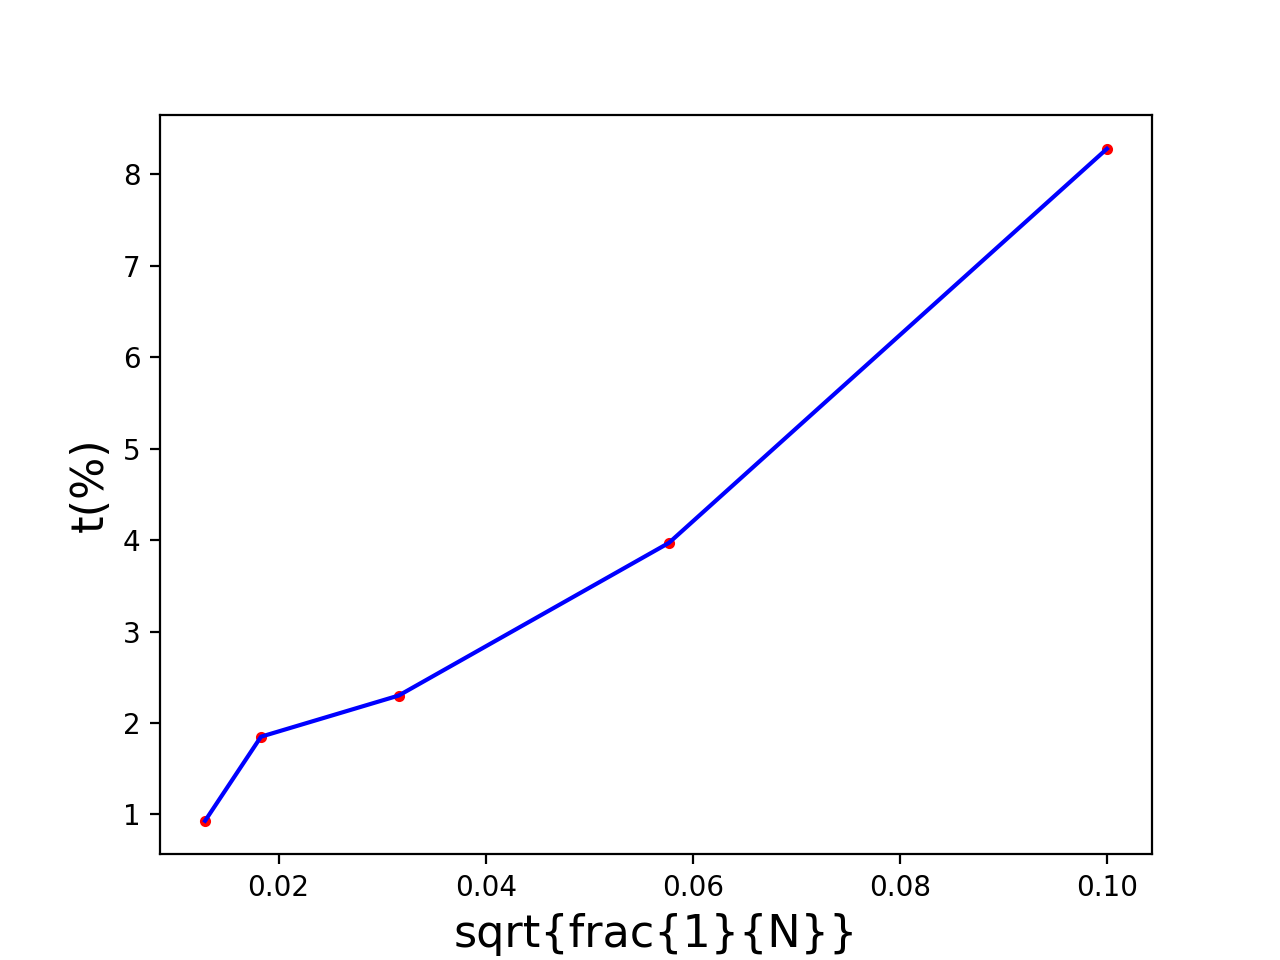
\includegraphics[width=0.7\textwidth]{linear1}
\end{figure}

\begin{figure}[!htbp]
\centering
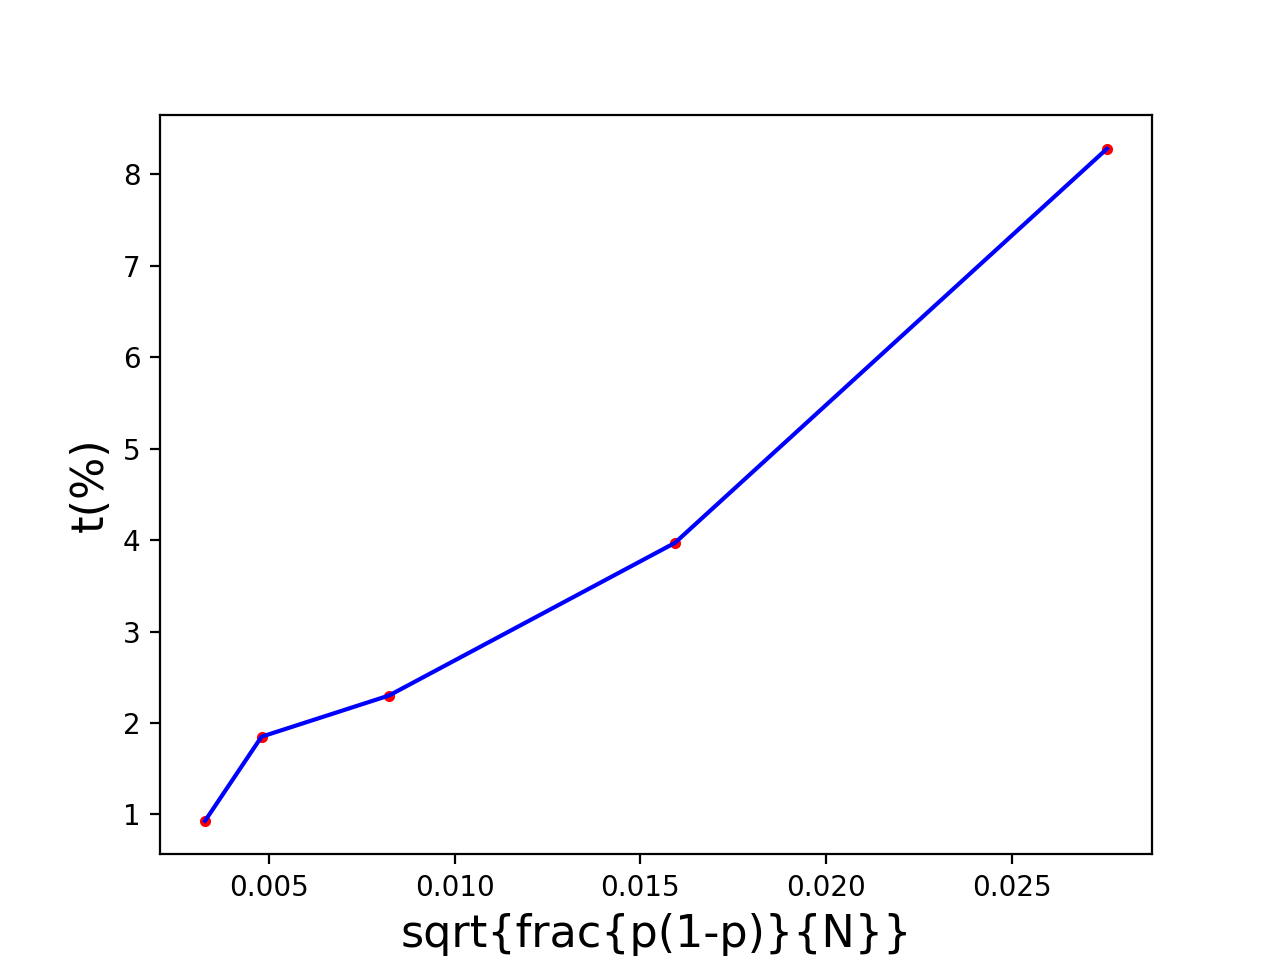
\includegraphics[width=0.7\textwidth]{linear2}
\end{figure}
\newpage